\section{Introduction to radio interferometric imaging}\label{radio}
In radio astronomy, there are two classes of radio sources: Point sources and extended emissions. Point sources are typically far-away stars, their emission is concentrated around a single pixel in the observed image. Extended emissions are objects that span a large area of the sky, like dust or hydrogen clouds. They span an area over several pixels. Both classes emit radio waves. The radio waves travel to earth, may get distorted by Earths Ionosphere, and finally arrive at the interferometer. Figure \ref{intro:system} shows the radio interferometry system.

\begin{figure}[h]
	\centering
	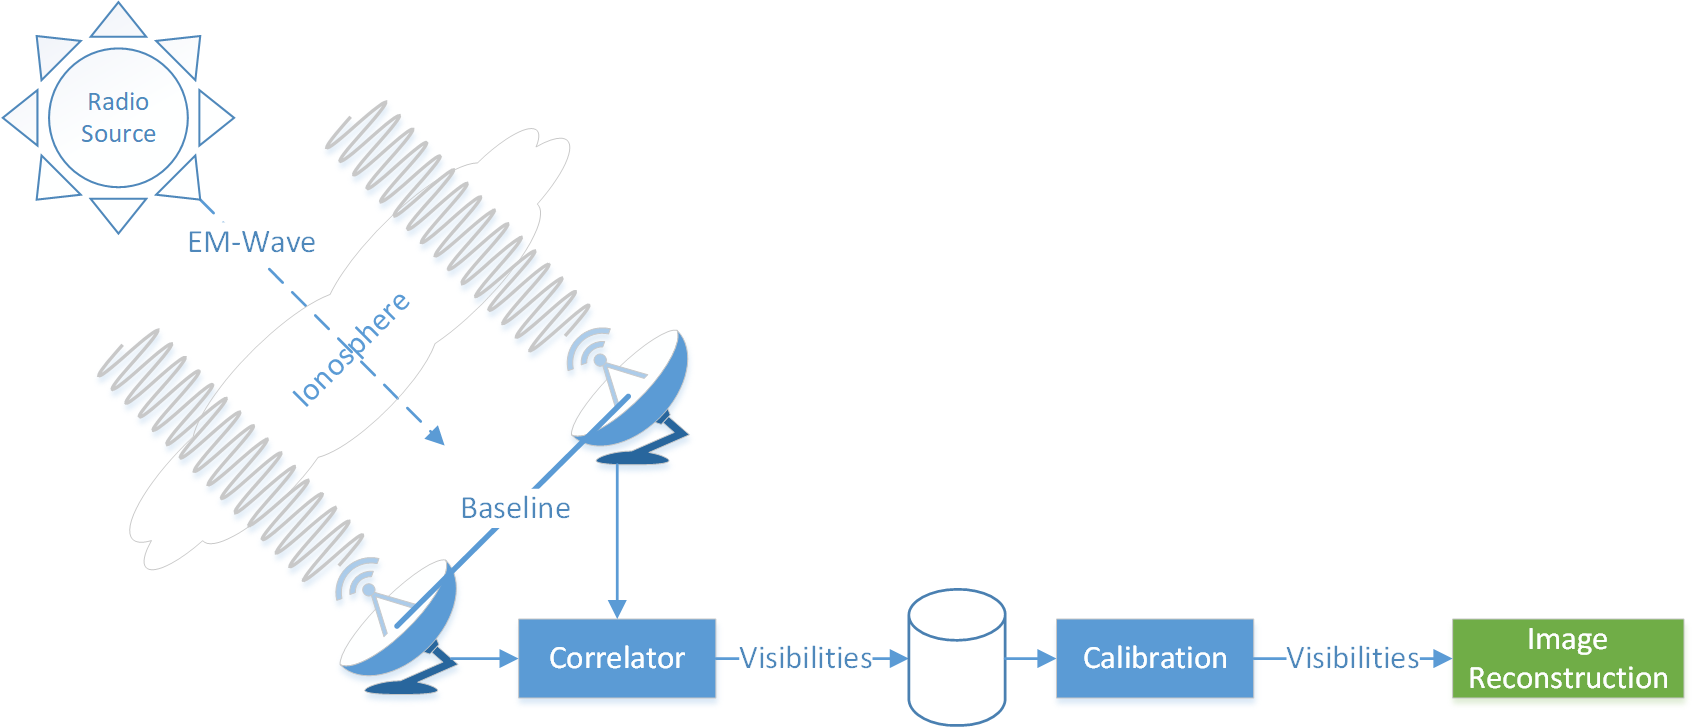
\includegraphics[width=0.80\linewidth]{./chapters/01.intro/system.png}
	\caption{Radio interferometry system}
	\label{intro:system}
\end{figure}

The electromagnetic waves arrive at the multiple antennas of the interferometer. The antennas are spaced apart from each other. Each antenna pair forms a 'baseline', which is the distance between the two antennas. Each antenna measures the electromagnetic waves independently of each other. The Correlator then takes the signal from each antenna pair (for each baseline), and correlates the signals. The correlator creates the complex visibility measurement for each baseline, consisting of an amplitude and phase measurement. After this step, the visibilities are saved for later reconstruction.

Before the visibilities can be reconstructed into an image, they need to be calibrated. Each antenna has a different sensitivity, which influences the amplitude and phase of the visibility measurements. Also, Earths Ionosphere can introduce noise to the amplitude and phase of each visibility measurement. In the calibration step, we estimate the different antenna gains, and influence by the Ionosphere and correct the visibility measurements. However, the calibration is imperfect. The image reconstruction step is tasked to find the most likely image from noisy and incomplete visibilities.

This project is focused on the image reconstruction step. We will develop our own image reconstruction algorithm that finds the most-likely image given the calibrated visibility measurements. However, the specifics of radio interferometric measurements influence every part of the image reconstruction algorithm. Efficient reconstruction algorithms have to deal with the specifics of radio interferometry. 

This section first introduces how image reconstruction works in theory. Then, we introduce the MeerKAT radio interferometer, for which we have real-world visibility measurements. We show the difficulties the MeerKAT interferometer introduces for the image reconstruction. Finally, we show how real-world image reconstruction algorithms work to deal with MeerKAT data, and show where our contributions lie.


\subsection{Introduction to the ill-posed inverse problem}\label{radio:cs}
Radio interferometers like MeerKAT generally produce more visibility measurements than pixels in the reconstruction. Still, the measurements are incomplete, and from the measurements alone, we cannot reconstruct the observed image. In the literature this is known as an ill-posed inverse problem. We wish to find the observed image from measurements in the Fourier space, but the measurements alone do not contain all the relevant information. 

First, we formulate the image reconstruction as a minimization problem with the following objective function:

\begin{equation}\label{radio:cs:l2}
\underset{x}{minimize} \: \left \| V - MFx \right \|_2^2
\end{equation}

Where $x$ is the reconstructed image we wish to find, $V$ are the measured visibilities, $F$ is the Fourier transform matrix and $M$ is the masking matrix. The masking matrix sets the visibilities that were are missing in the image. 

We can reconstruct the image by finding the optimum of the objective function \eqref{radio:cs:l2}. The objective function is convex, meaning it has only one global minimum, and we can use the class of convex optimization algorithms to search the minimum. However, our measurements $V$ are incomplete, meaning we do not have all the data we need for reconstruction. This means our objective function \eqref{radio:cs:l2} does not "point" to the observed image. It still has a global minimum, but observed image is not guaranteed to be near the global minimum. 

A side note: We are guaranteed to find the observed image at the minimum of \eqref{radio:cs:l2} is when the measurements fulfill the Nyquist-Shannon sampling theorem. In that case, we can find the minimum by calculating the inverse Fourier transform: $x = F^{-1}V$. We can still calculate the inverse Fourier transform when we are dealing with incomplete measurements, but it does not result in the observed image.

The objective \eqref{radio:cs:l2} only includes information about the measurements. As we have mentioned before, we have prior knowledge about the image. We know for example it is likely to contain point sources. In that case, most pixels of the image will be zero, except for the locations where the interferometer has located the point sources. In other words, we know that the image is sparse. We can add a regularization to the objective function \eqref{radio:cs:l2}, which models this prior information and forces the reconstructed image to be sparse (contain as few non-zero pixels as possible ). This results in the modified objective function:

\begin{equation}\label{radio:cs:lasso}
\underset{x}{minimize} \: \left \| V - MFx \right \|_2^2 + \lambda \left \| x \right \|_1
\end{equation}

Note the two terms in the objective \eqref{radio:cs:lasso}: We have the same term from our measurements, which we call the "data term". But we also have an additional "regularization term", which is the L1 norm\footnote{Sum of absolute values of the pixels, $\sum_i \sum_j \left \| x_{ij} \right \|$} and forces our reconstruction to be sparse. The parameter $\lambda$ represents how much emphasis we put on the regularization. The new objective function is still convex, it still has a global minimum. The regularization term simply shifted the global minimum to a different location when compared to the first objective \eqref{radio:cs:l2}. Now the question is: Does it point to the observed image? In practice, if the regularization is a good model for the image content, the reconstructed image found at the minimum of \eqref{radio:cs:lasso} is indistinguishable from the observed image.

In reality, no regularization models the image content perfectly. The L1 regularization for example does not account for extended emissions, when we have a large area of non-zero pixels. In this case, the reconstructed image found at the minimum of \eqref{radio:cs:lasso} has visible differences to the truly observed image. The regularization is responsible for the 'reconstruction quality', how close the reconstructed image is to the truly observed one.

In a sense there is data modeling task involved in the image reconstruction. The better we understand what a plausible image looks like, the higher the reconstruction quality. Recent work managed to reconstruct super-resolved images for the VLA interferometer\cite{dabbech2018cygnus}, where the reconstruction achieved a resolution higher than the limit of the instrument itself.

The image reconstruction problem is ill-posed, but with the right regularization we can reconstruct an image which even surpasses the accuracy limit of the instrument. However, the regularization also influences other properties of the reconstruction algorithm, such as the wall-clock time for a single reconstruction, or its behavior with very noisy visibilities. The question of the optimal regularization is, as of the time of writing, still open in radio astronomy.


\subsection{Introduction to the MeerKAT observations}
So far, we looked at how image reconstruction works in theory. We need a regularization to model our prior knowledge, that the image is a mixture of point sources and extended emissions. Then, all we need is a convex optimization algorithm, which finds us the most likely image. Real-world radio interferometer introduce complexities which have to be handled by the reconstruction algorithm. First, there is a large number of visibility measurements. Any operation on the measurements is potentially time consuming. Secondly, the measurements of modern radio interferometers become more complicated, as we will show in the next section. Here, we show how MeerKAT can produce an almost arbitrary large amount of visibility measurements.

\begin{figure}[!h]
	\centering
	\begin{subfigure}[b]{0.4\linewidth}
		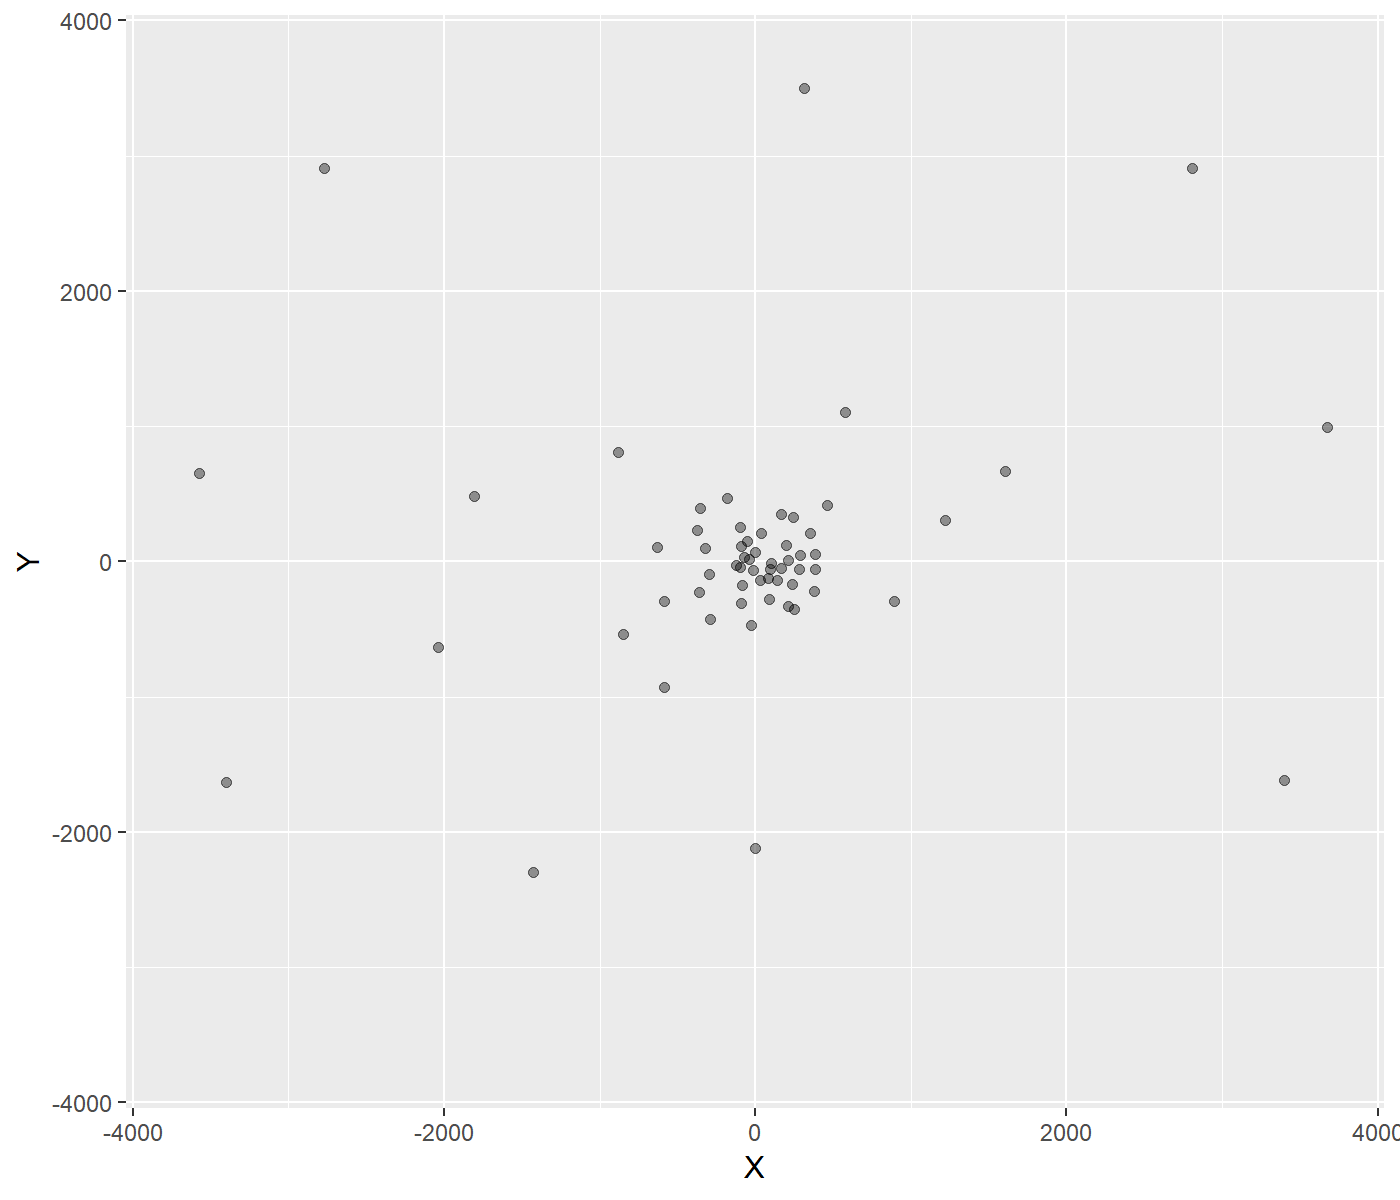
\includegraphics[width=\linewidth]{./chapters/01.intro/aperture/ants.png}
		\caption{Antenna layout.}
		\label{radio:sampling:ants}
	\end{subfigure}
	\begin{subfigure}[b]{0.4\linewidth}
		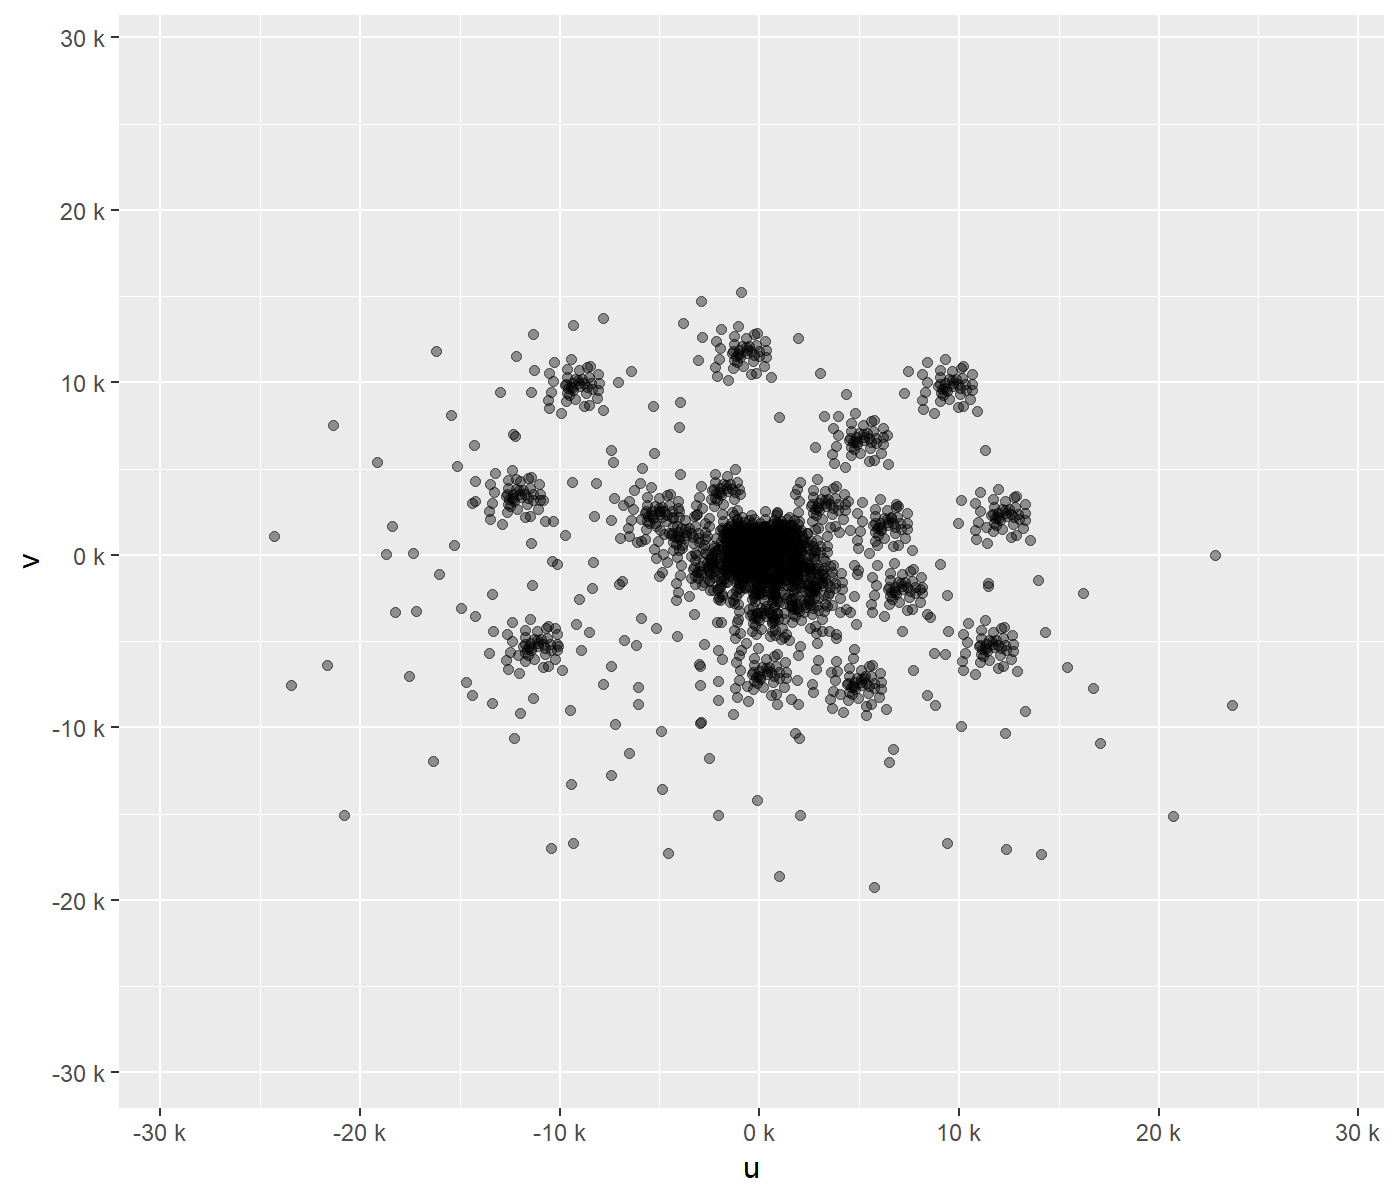
\includegraphics[width=\linewidth]{./chapters/01.intro/aperture/snapshot.png}
		\caption{Visibility sampling pattern.}
		\label{radio:sampling:pattern}
	\end{subfigure}
	\\
	\begin{subfigure}[b]{0.4\linewidth}
		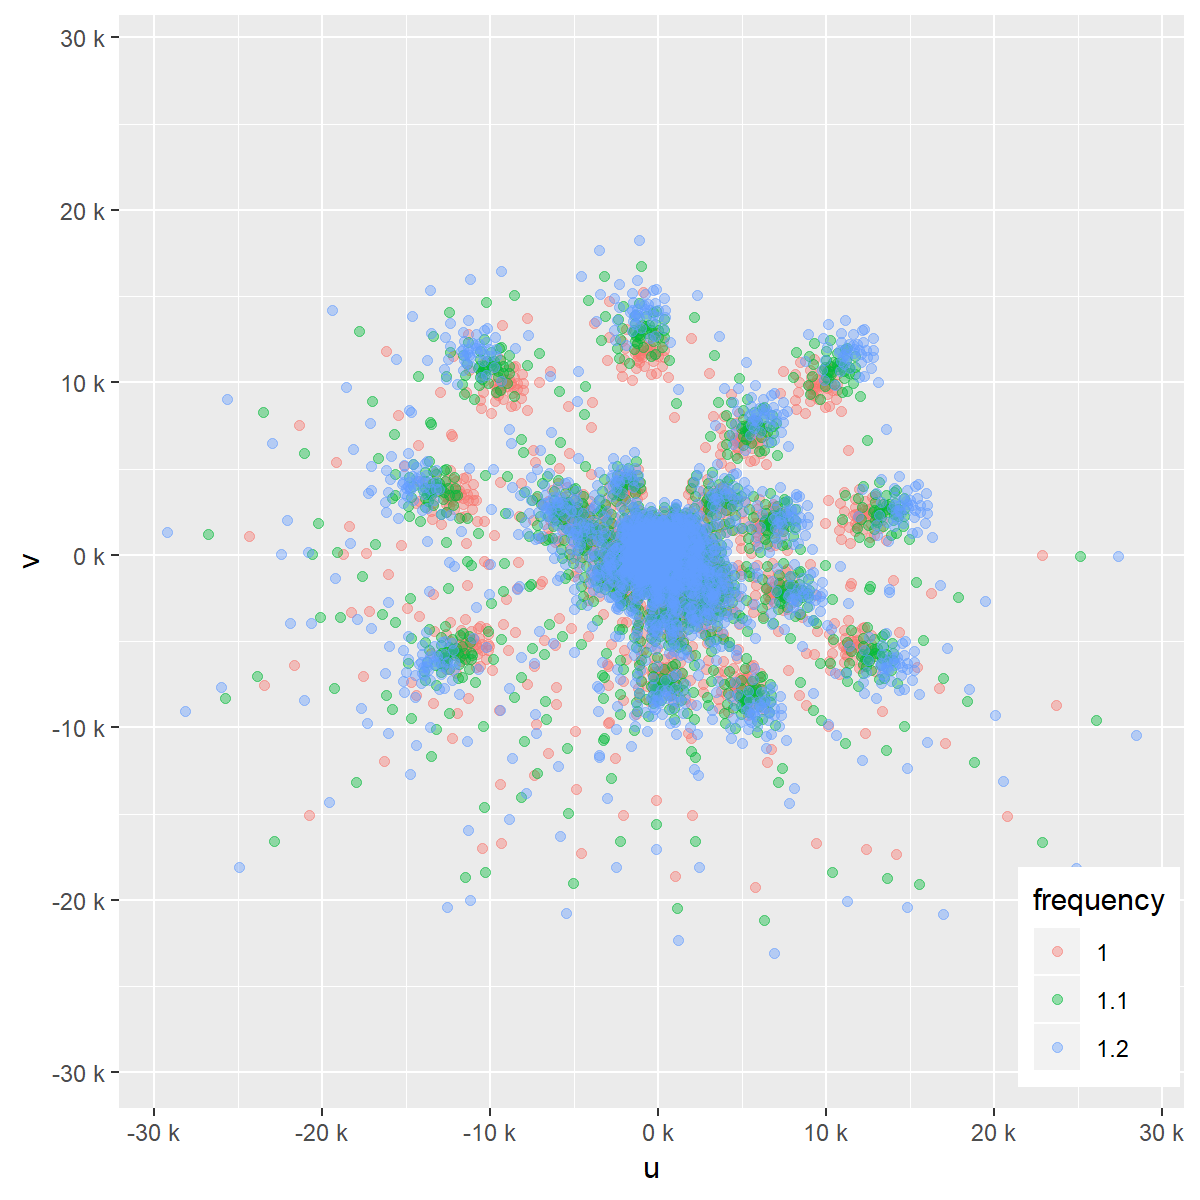
\includegraphics[width=\linewidth]{./chapters/01.intro/aperture/frequencies.png}
		\caption{Visibilities added from multiple channels.}
		\label{radio:sampling:freq}
	\end{subfigure}
	\begin{subfigure}[b]{0.4\linewidth}
		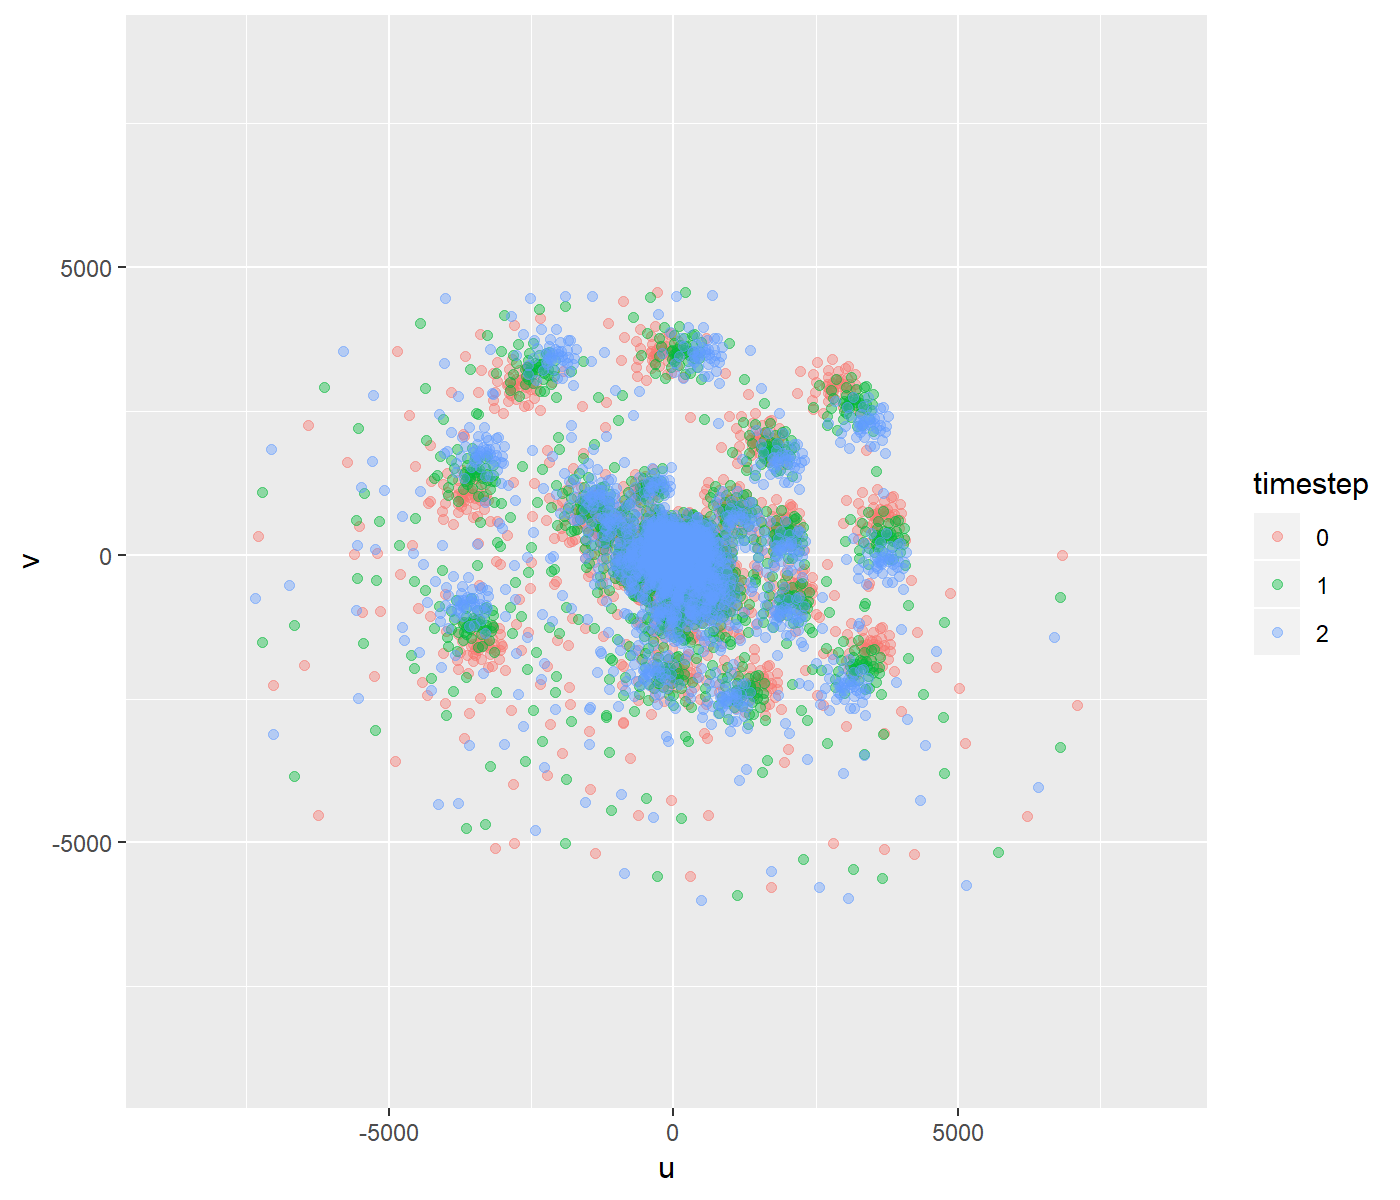
\includegraphics[width=\linewidth]{./chapters/01.intro/aperture/timesteps.png}
		\caption{Visibilities added from multiple timesteps.}
		\label{radio:sampling:time}
	\end{subfigure}
	
	\caption{Sampling regime of the MeerKAT radio interferometer.}
	\label{intro:sampling}
\end{figure}


The MeerKAT radio interferometer consists of 64 antennas. Each antenna pair is a single baseline of the interferometer, which results in a single visibility measurement. This leads to 2016 visibilities for the MeerKAT interferometer. The distance between the antennas of each pair is important: The distance defines what point in the Fourier space gets sampled. A short baseline samples close to the origin of the Fourier space, and contain low-frequency Fourier components of the sky image. Long baselines measure points further away from the origin. They sample the high-frequency Fourier components, and contain information about sharp edges in the image. Figure \ref{radio:sampling:ants} shows the 64 antennas of MeerKAT, while the Figure \ref{radio:sampling:pattern} shows the 2016 visibility samples in the Fourier space.

The sampling pattern of the MeerKAT interferometer is not uniform in the Fourier space. We have areas which are densely sampled, and areas which are sparsely sampled. Note that we only have a few samples of the high-frequency Fourier components. We are missing measurements from a large portion of the Fourier space. Modern radio interferometers use two tricks to fill up the Fourier space with more visibility samples: Adding visiblities from different channels, and from different timesteps.

The interferometer measures the sky at different wavelengths simultaneously. We can add the visibilities from neighboring channels together, resulting in the visibility pattern shown in Figure \ref{radio:sampling:freq}. Each channel measures the Fourier space using the same pattern, but scaled by the radio frequency.

The interferometer observes the sky over a period of time. Depending on the observation, this can be minutes, up to several hours. During this time, the rotation of the Earth rotates the sampling pattern in Fourier space, shown in Figure \ref{radio:sampling:time}.

The MeerKAT radio interferometer measures 2016 visibilities, for each channel at each timestep. It has 20 thousand channels, and the time resolution can be as low as half a second. This results in roughly 80 million visibility measurements for each second of observation. A real-world observation can span over several hours, and take up several terabytes of disk space. The data volume alone creates difficulties in any practical reconstruction algorithm. The large number of visibility measurements is difficult to keep in memory. Any operation on the whole set of visibilities becomes impractical.

But MeerKAT introduces further complications apart from the large data volume. Adding the visibilities from 20 thousand channels together becomes inaccurate. For an accurate reconstruction, the reconstruction algorithm has to perform wide-band imaging: Instead of reconstructing a single image containing the visibilities from all frequencies, the algorithm reconstructs an image cube, where each image represents a single, or a small fraction of all channels. Wide-band imaging is out of scope for our project, and our reconstruction algorithm only considers narrow-band imaging.

Furthermore, the reconstructed image from MeerKAT observations generally span a wide field-of-view. For an accurate reconstruction, the algorithm has to account for the fact that the visibilities are three dimensional. We include wide field-of-view imaging in our reconstruction algorithm, and discuss the effects of the third visibility term in more detail.


\subsubsection{Introduction to the third visibility term}
As we discussed so far, the radio interferometer measures visibilities of the sky image, and we wish to find the observed image from the measurements. We have ignored the fact that the visibility measurements not only have a $u-$ and $v$-, but also a third $w$-term. Visibilities are in fact three dimensional. The third $w$ component arises from the fact that the baselines (antenna pairs) are not on the same plane. The curvature of the earth, local hills and other terrain feature introduce the $w$-term. The $w$-term becomes relevant for wide field-of-view imaging in radio interferometry. Let us start with the measurement equation for small field-of-views:

\begin{equation}\label{intro2:model:smallfov}
V(u, v) = \int\int I(l, m)  e^{2 \pi i [ul+vm]} \: dl \: dm
\end{equation}

The radio interferometer measures Visibilities $V$ from the sky image $I$. Each visibility is a measurement over all pixels $l, m$. The term $ e^{2 \pi i [ul+vm]}$ is simply the Fourier transform. $l$ and $m$ are the directions from which we measured radiation. They can be thought of as the pixel indices of the image. Index $(0,0)$ is the center pixel of the image. So far the visibilities are two dimensional. But this measurement equation is only valid for a small field-of-view. For a large field-of-view the measurement equation expands to:

\begin{equation}\label{intro2:model:widefov}
V(u, v, w) = \int\int  \frac{I(l, m)}{c(l, m)}  e^{2 \pi i [ul+vm + w(c(l, m) - 1)]} \: dl \: dm \:,  \quad c(l,m) = \sqrt{1 - l^2 - m ^2}
\end{equation} 

We still have the Fourier transform $ e^{2 \pi i [ul+vm \ldots]}$ at the core. But now the visibilities have a third $w$-term, the image has a normalization factor of $c(l, m)$ and the Fourier transform has a phase-shift $+ w(c(l, m) - 1)$ added to it. The phase-shift of the Fourier transform depends on the direction from which the radiation was measured. As such, the phase shift changes over the image. It is called a Directionally Dependent Effect (DDE).

There exist several sources of DDE's. The Ionoshpere for example is a natural source that distorts the signal depending on the direction. From different directions, the distortion by the Ionosphere changes. The $w$-term arises from the properties of the interferometer itself. DDE's are costly in terms of computation time. The $w$-term breaks the two dimensional Fourier relationship between the image and the visibilities. This creates a difficulty when we need to calculate the Fourier transform of the visibility measurements:  Calculating the Fourier transform for a large number of visibility measurements becomes expensive. The Fast Fourier Transform (FFT) is significantly faster. But we cannot use the FFT for the visibilities: It requires the visibilities sampled on a uniform grid, and does not expect a three dimensional Fourier space to result in a two dimensional image. 

Image reconstruction pipelines in radio astronomy solve these issues by using a 'gridder'. The gridder is tasked with interpolating the non-uniformly sampled visibilities on a uniform grid, and correcting for the $w$-term. The gridder creates a uniformly sampled Fourier grid, which then can be efficiently transformed into the image space with an FFT. In this project, we do not focus on the gridding algorithm. We implemented the gridder developed by Veenboer et al. \cite{veenboer2017image}. It is responsible for interpolating the visibilities and correcting for the $w$-term in an efficient manner.

The gridder lets us efficiently transform the visibility measurements into an image. But it does not shield the reconstruction algorithm from the DDE's themselves. As we will see, an image reconstruction algorithm also has to correct for DDE's during reconstruction. 


\subsection{Introduction to image reconstruction algorithm for radio interferometer}\label{intro2:rec}
This section introduces the commonly used architecture for radio interferometric image reconstruction, the Major/Minor cycle. It shows how DDE's like the $w$-term are handled, and introduces the basic reconstruction algorithm for radio astronomy: CLEAN.

First, let us look back at the objective function. In the previous section, the objective function \eqref{radio:cs:lasso} contained the visiblity measurements $V$ in Fourier space, the reconstructed image $x$ in image space, and the Fourier transform matrix $F$ that represents the relationship between image and Fourier space. However, this is only one way to formulate the reconstruction problem:

\begin{equation} \label{radio:rec:objective}
\begin{split}
\underset{x}{minimize} &\: \left \| V - MFx \right \|_2^2 + \lambda \left \| x \right \|_1 \\
\underset{V_2}{minimize} &\: \left \| V - MV_2 \right \|_2^2 + \lambda \left \| F^{-1}V_2 \right \|_1 \\
\underset{x}{minimize} &\: \left \| I_{dirty} - x * PSF \right \|_2^2 + \lambda \left \| x \right \|_1
\end{split}
\end{equation}

We can also reconstruct the missing visibilities directly. In that case, we solve an in-painting problem in the Fourier space. Or we can transform the measurements into image space, and solve an equivalent deconvolution problem, where the masking matrix $M$ in Fourier space becomes the convolution kernel called the Point Spread Function $PSF$ (Remember that a multiplication in Fourier space is a convolution in image space.)

These three problems are equivalent in theory. The key difference between the three formulations is that the we generally have magnitudes fewer pixels than visibility measurements in the reconstruction problem. The deconvolution problem takes up less physical memory, and is therefore easier to handle in practice.

Image reconstruction algorithms for radio interferometers generally use the deconvolution formulation. They first transform the visibility measurements to an image, called the dirty image. The gridder first interpolates the visibilities, and the FFT calculates the final dirty image. Then, they transform the masking matrix $M$ into the image space, which results in the $PSF$. At this point, the algorithms reconstruct the image by calculating a deconvolution. Figure \ref{radio:alg:figure} shows a simulated example of a dirt image, $PSF$ and deconvolved image.

\begin{figure}[h]
	\centering
	\begin{subfigure}[b]{0.3\linewidth}
		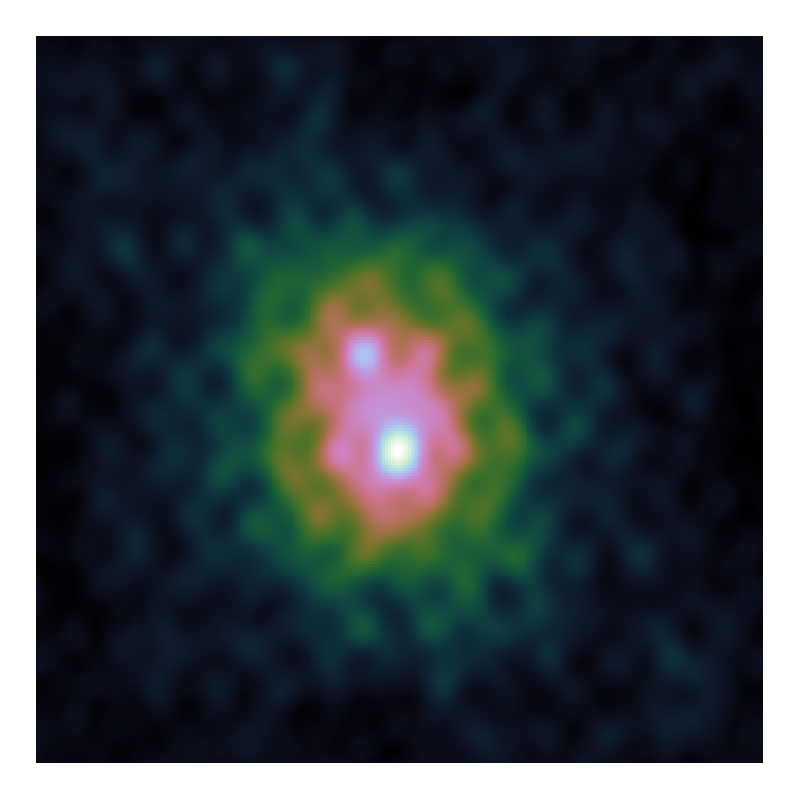
\includegraphics[width=\linewidth, clip, trim= 0.25in 0.25in 0.25in 0.25in]{./chapters/03.cd/simulated/dirty.png}
		\caption{Dirty Image.}
		\label{radio:alg:dirty}
	\end{subfigure}
	\begin{subfigure}[b]{0.3\linewidth}
		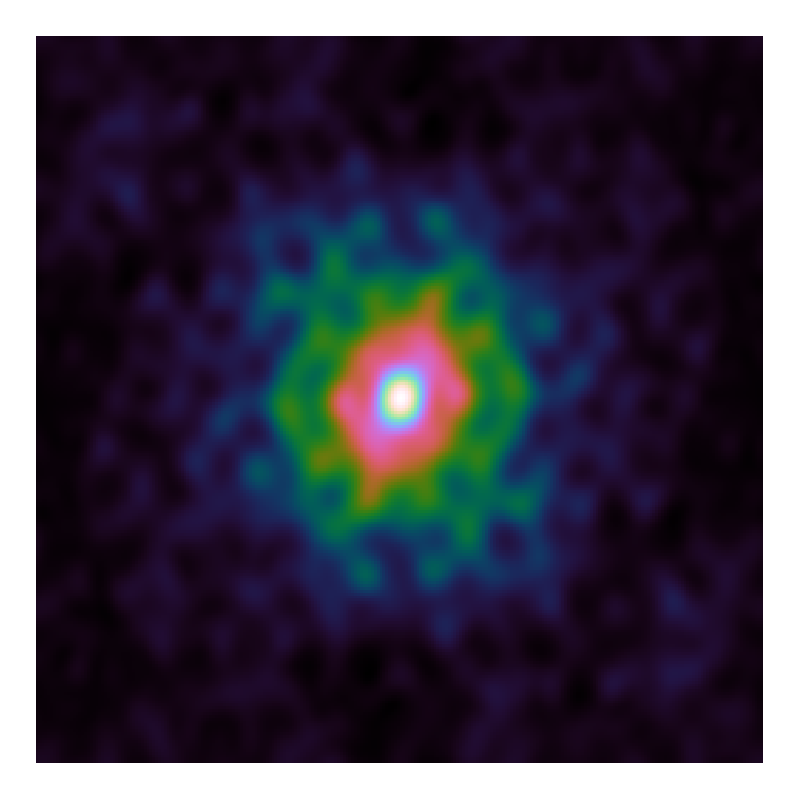
\includegraphics[width=\linewidth, clip, trim= 0.25in 0.25in 0.25in 0.25in]{./chapters/03.cd/simulated/psf.png}
		\caption{Point Spread Function.}
		\label{radio:alg:psf}
	\end{subfigure}
	\begin{subfigure}[b]{0.3\linewidth}
		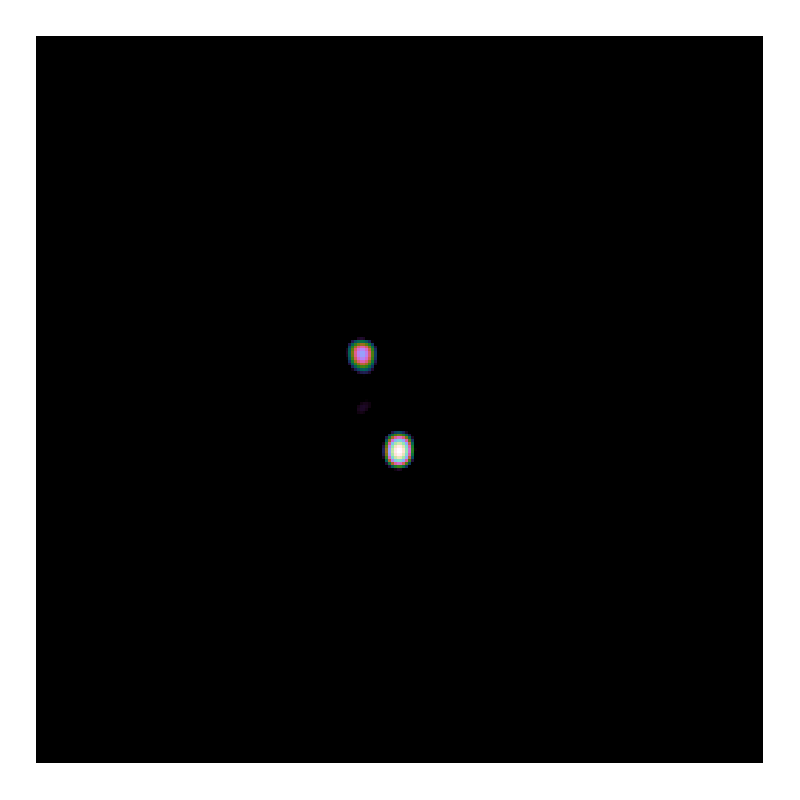
\includegraphics[width=\linewidth, clip, trim= 0.25in 0.25in 0.25in 0.25in]{./chapters/03.cd/simulated/elasticNet.png}
		\caption{Deconvolution}
		\label{radio:alg:elastic}
	\end{subfigure}

	\caption{Example deconvolution problem with two point sources.}
	\label{radio:alg:figure}
\end{figure}

In radio astronomy, image reconstruction is split into two separate algorithms. The first algorithm is responsible for transforming the measurements from Fourier to image space. The second algorithm is responsible for deconvolution. The first algorithm is referred as the Major cycle in radio astronomy, and the deconvolution algorithm as the minor cycle in radio astronomy literature. The reason why they are referred to as "cycles" will become clear in Section \ref{intro2:opt:cycle}. In short: The whole process, transforming the measurements to image space and calculating the deconvolution has to be repeated several times to correct for DDE's like the $w$-term. First, we will take a closer look to the most commonly used deconvolution algorithm, CLEAN.


\subsubsection{CLEAN deconvolution algorithm} \label{intro2:CLEAN}
CLEAN\cite{hogbom1974aperture} is the basic deconvolution algorithm in radio astronomy. It has been extended over the years, and in its more sophisticated form as multi-scale multi-frequency CLEAN \cite{offringa2017optimized} is still used today. We introduce the basic CLEAN algorithm in this section.

The CLEAN deconvolution algorithm keeps three images in memory: The residual image, the model image, and the $PSF$. In general, all three images are the same size. At the start of the algorithm, the residual image is equal to the dirty image shown in Figure \ref{radio:alg:dirty}. The model image starts with every pixel set to zero. It is updated in each iteration and will, at the end, contain the deconvolved version of the dirty image.

A CLEAN iteration begins with searching the maximum pixel in the residual image. In the next step, it adds a fraction of the maximum value to the model image. For example, if the maximum pixel is 2.7, CLEAN adds 1.35 to the model image at the same location (This fraction is called the CLEAN gain and is one of the parameters left for the user to define). The last step is to subtract the $PSF$ at the location. The Figure \ref{radio:clean:figure} shows the residual and the model image over four iterations.

\begin{figure}[h]
	\centering
	\begin{subfigure}[b]{0.48\linewidth}
		\begin{subfigure}[b]{0.48\linewidth}
			\centering
			Residuals\\
			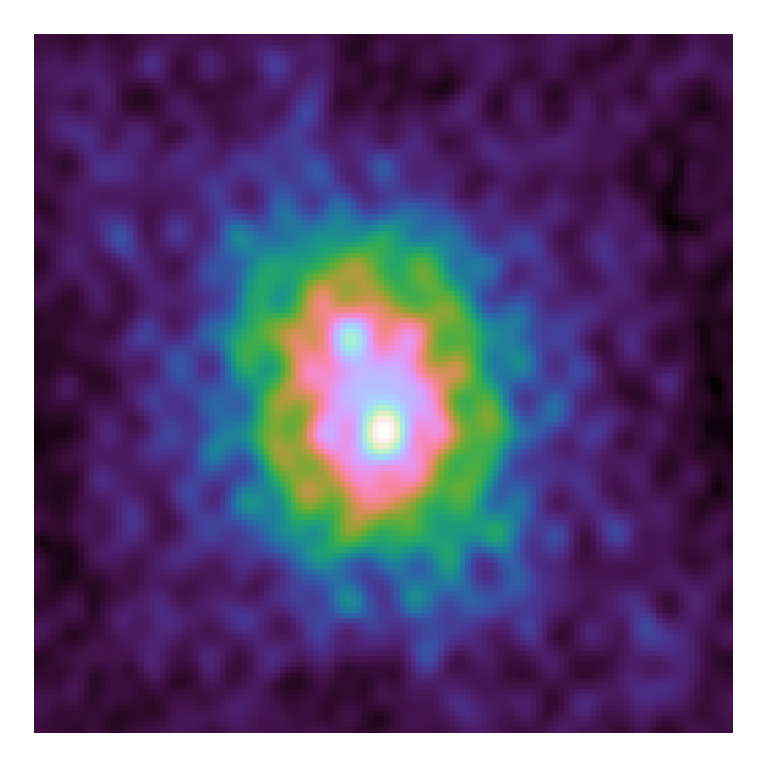
\includegraphics[width=1.0\linewidth, clip, trim= 1.0in 1.0in 1.0in 1.0in]{./chapters/01.intro/cleanExample/dirty_CLEAN_0.png}
		\end{subfigure}
			\begin{subfigure}[b]{0.48\linewidth}
			\centering
			Model\\
			
\includegraphics[width=1.0\linewidth, clip, trim= 1.0in 1.0in 1.0in 1.0in]{./chapters/01.intro/cleanExample/model_CLEAN_0.png}
		\end{subfigure}
		\caption{Iteration 0}
	\end{subfigure}
	\begin{subfigure}[b]{0.48\linewidth}
		\begin{subfigure}[b]{0.48\linewidth}
			\centering
			Residuals\\
			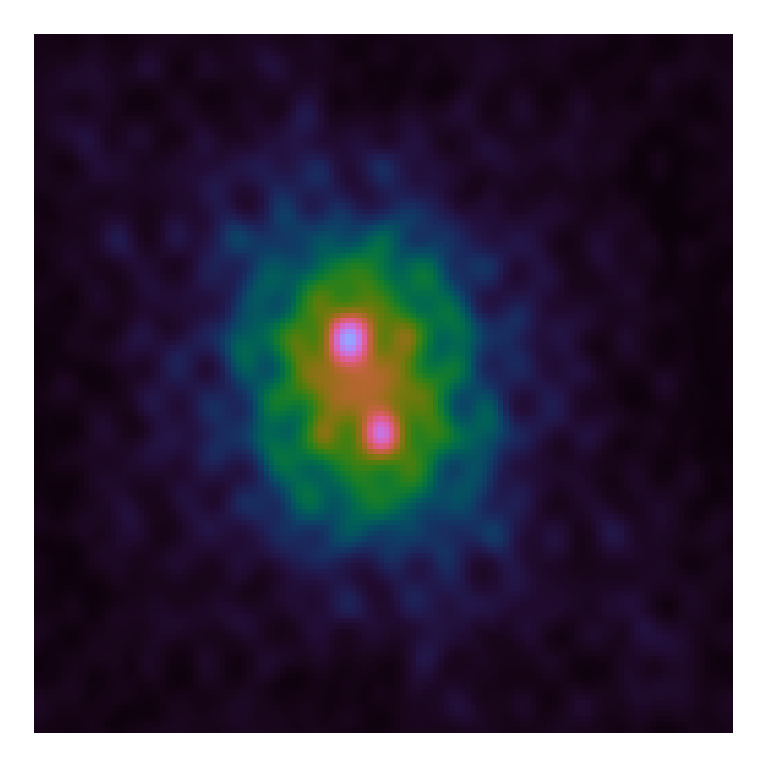
\includegraphics[width=1.0\linewidth, clip, trim= 1.0in 1.0in 1.0in 1.0in]{./chapters/01.intro/cleanExample/dirty_CLEAN_1.png}
		\end{subfigure}
		\begin{subfigure}[b]{0.48\linewidth}
			\centering
			Model\\
			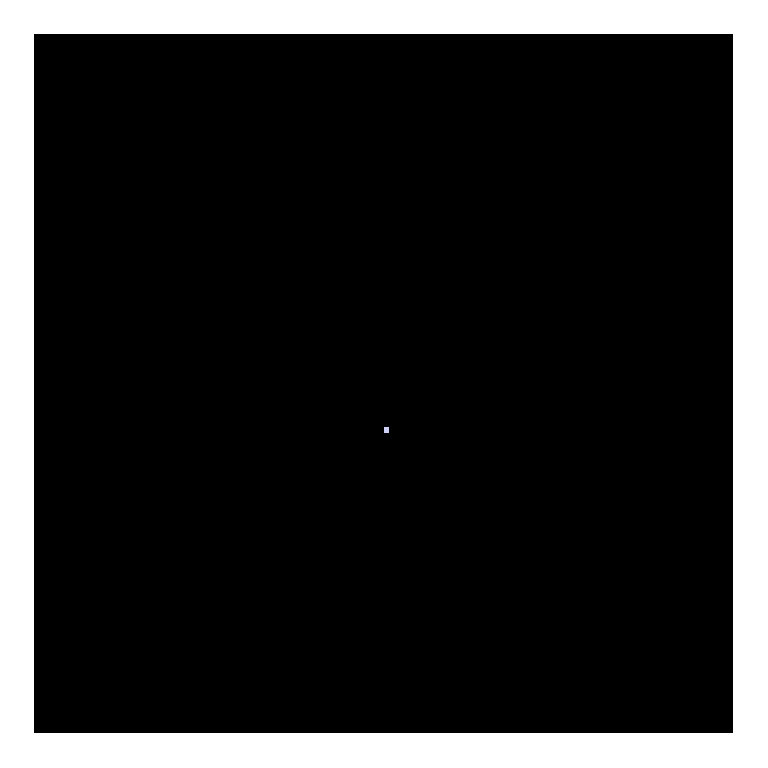
\includegraphics[width=1.0\linewidth, clip, trim= 1.0in 1.0in 1.0in 1.0in]{./chapters/01.intro/cleanExample/model_CLEAN_1.png}
		\end{subfigure}
		\caption{Iteration 1}
	\end{subfigure}
	\begin{subfigure}[b]{0.48\linewidth}
		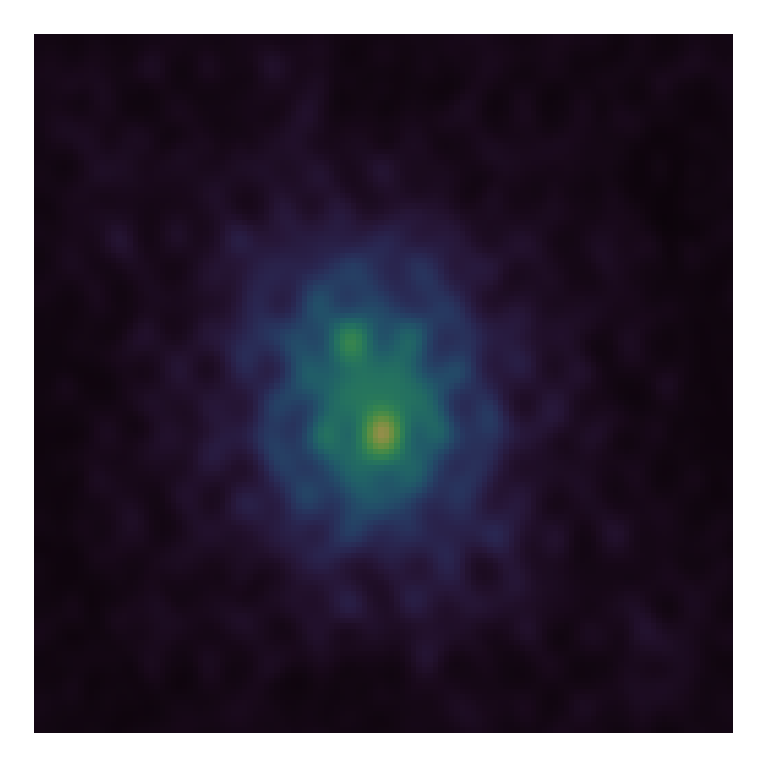
\includegraphics[width=0.48\linewidth, clip, trim= 1.0in 1.0in 1.0in 1.0in]{./chapters/01.intro/cleanExample/dirty_CLEAN_2.png}  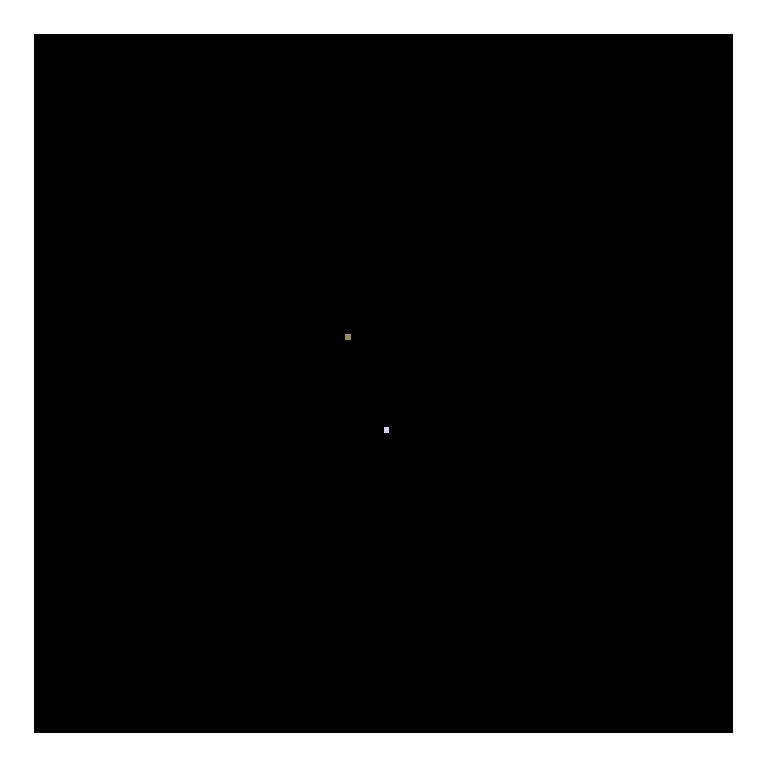
\includegraphics[width=0.48\linewidth, clip, trim= 1.0in 1.0in 1.0in 1.0in]{./chapters/01.intro/cleanExample/model_CLEAN_2.png} 
		\caption{Iteration 2}
	\end{subfigure}
	\begin{subfigure}[b]{0.48\linewidth}
		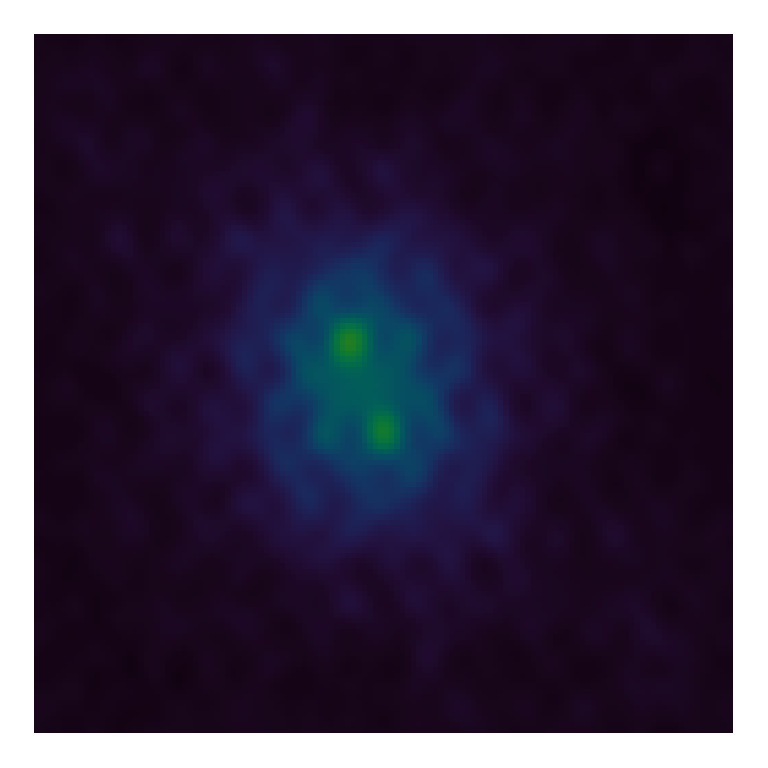
\includegraphics[width=0.48\linewidth, clip, trim= 1.0in 1.0in 1.0in 1.0in]{./chapters/01.intro/cleanExample/dirty_CLEAN_3.png}  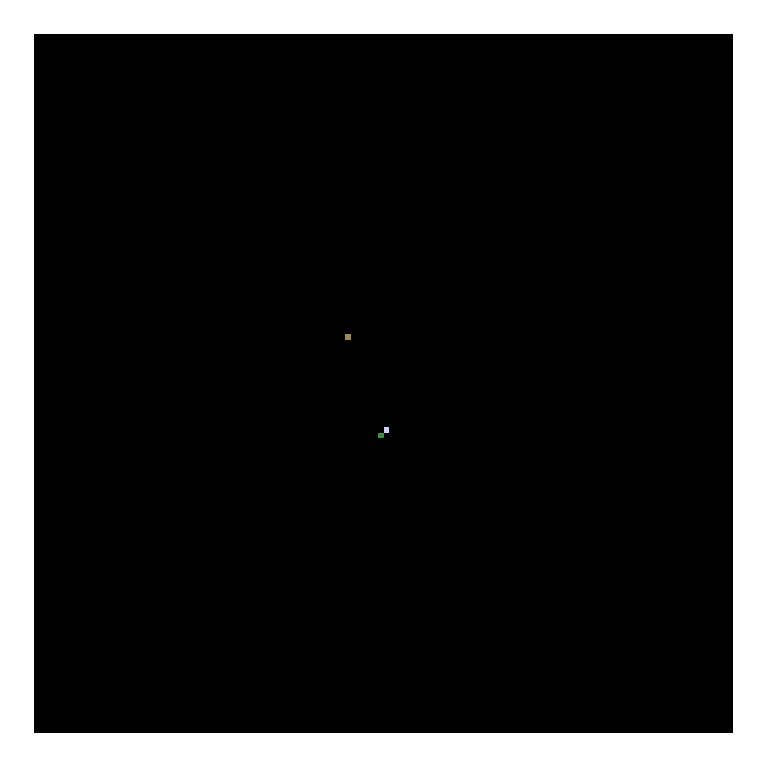
\includegraphics[width=0.48\linewidth, clip, trim= 1.0in 1.0in 1.0in 1.0in]{./chapters/01.intro/cleanExample/model_CLEAN_3.png} 
		\caption{Iteration 3}
		\label{radio:clean:figure:iter3}
	\end{subfigure}

	\caption{CLEAN deconvolution iterations.}
	\label{radio:clean:figure}
\end{figure}

After a number of CLEAN iterations, the model image contains a number of non-zero pixels. But CLEAN also leaves artifacts in the model image. As we see in Figure \ref{radio:clean:figure:iter3}, iteration 3 adds another non-zero pixel close to the already detected one. CLEAN brushes over the artifacts by simply blurring the model image with the "CLEAN-beam" after CLEAN has finished its iterations. The CLEAN-beam represents the accuracy limit of the radio interferometer. By blurring the image, CLEAN reconstructs the image at the limit of the instrument. The blurring with the CLEAN-beam is shown in Figure \ref{radio:clean:beam}

\begin{figure}[h]
	\centering
	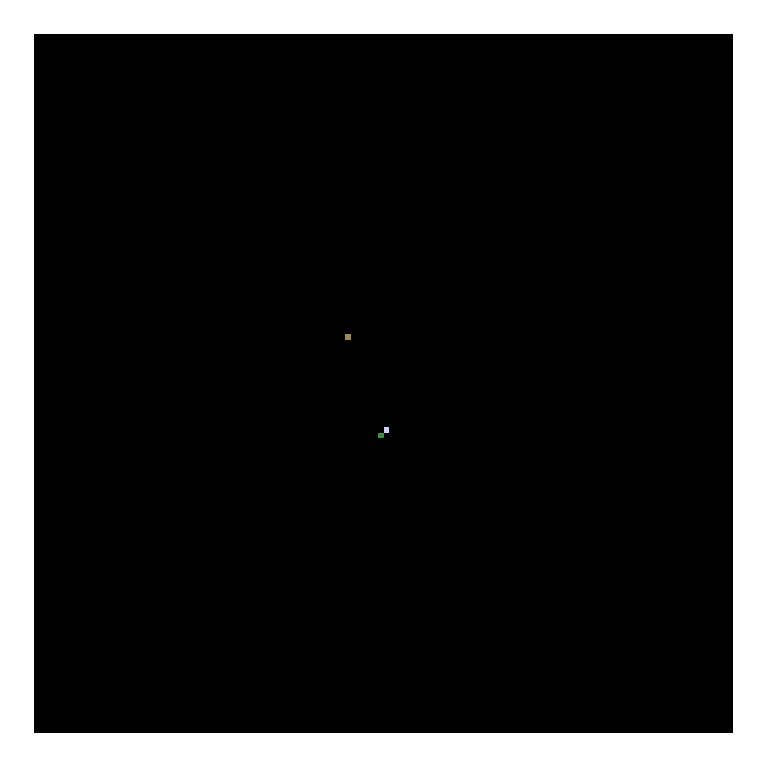
\includegraphics[width=0.25\linewidth, clip, trim= 1.0in 1.0in 1.0in 1.0in]{./chapters/01.intro/cleanExample/model_CLEAN_3.png}
	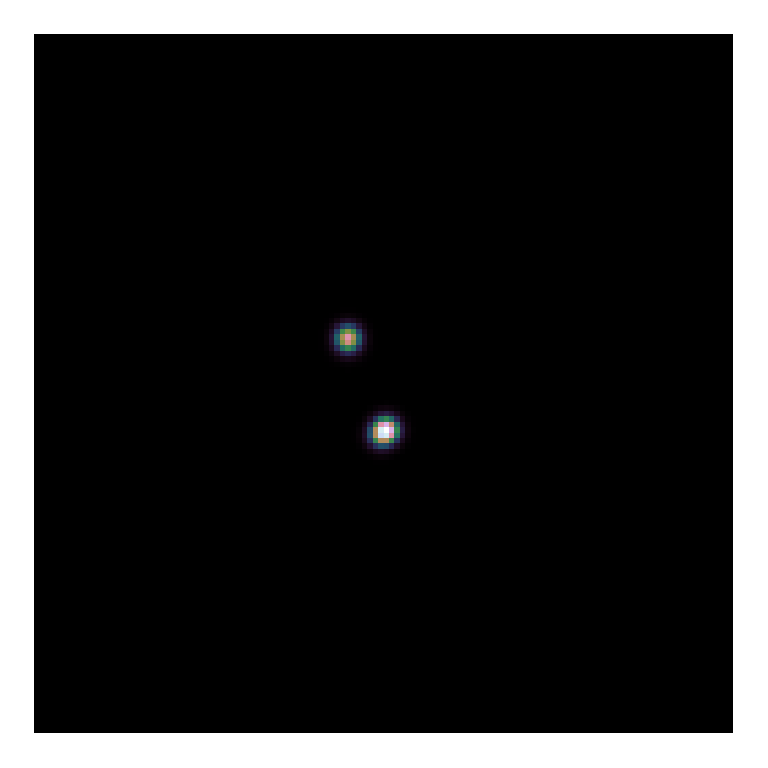
\includegraphics[width=0.25\linewidth, clip, trim= 1.0in 1.0in 1.0in 1.0in]{./chapters/01.intro/cleanExample/rec_CLEAN.png}
	\caption{Blurring with the CLEAN-beam}
	\label{radio:clean:beam}
\end{figure}

The CLEAN algorithm assumes the image contains point sources. In each iteration, it essentially adds the most-likely point source. It is a greedy algorithm, because it searches the most-likely point source in each iteration. The objective function which CLEAN is minimizing is similar to the deconvolution objective function \eqref{radio:rec:objective}: The difference is CLEAN does not use the L1 regularization, but the L0 'norm':

\begin{equation}\label{radio:clean:l0}
\underset{x}{minimize} \: \left \| V - MFx \right \|_2^2 + \lambda \left \| x \right \|_0
\end{equation}

The reconstructed image $x$ is equivalent to the model image from Figure \ref{radio:clean:figure}. L0 'norm' in this context means the indicator function. The indicator function is 1 for every element of $x$ which is non-zero.  We call it the L0 'norm', because it is used as a norm in signal processing, but does not fulfill all properties of a norm in Linear Algebra.   The L0 'norm' and the L1 are related: Both enforce sparsity in the reconstructed image $x$. But where the L1 norm results in a convex objective function with a unique optimum, the L0 'norm' results in a non-convex objective, possibly with local minima and no guaranteed unique minimum. 

L1 norm is the convex relaxation of the L0 'norm'. In practice, the L0 regularized objective function \eqref{radio:clean:l0} and the L1 regularized objective function \eqref{radio:cs:lasso} almost always lead to the same reconstructed image \cite{candes2006robust}\cite{donoho2006compressed}. But for the L0 regularized objective, we need an algorithm from the class of non-convex optimization methods. Real-world CLEAN implementations use additional strategies to speed up convergence, or improve the quality of the restored image. A specific CLEAN implementation only approximately minimizes the L0 regularized objective \eqref{radio:clean:l0}. Still, the CLEAN algorithm belongs to the class of non-convex optimization algorithms.

In this project, we focus on convex objective functions. We develop two coordinate descent based deconvolution algorithms, which belong to the class of convex optimization.


\subsubsection{The Major/Minor cycle}\label{intro2:opt:cycle}
During CLEAN deconvolutions, the algorithm assumes that the $PSF$ is constant over the image. However, this is not the case for wide field-of-view observations. The $w$-term changes the $PSF$ depending on the location in the image. CLEAN deconvolutions only approximate the true $PSF$. With more CLEAN iterations, the residuals image becomes less accurate. To solve this issue, a deconvolution algorithm is used inside the Major/Minor cycle framework. 

The Minor cycle is responsible for deconvolution. Typically, a CLEAN based algorithm is used. Every CLEAN iteration is refferred to as one Minor cycle. After a number of CLEAN iterations, the residual image is too inaccurate. Then, the Major cycle takes the model image of CLEAN, and transforms it back to the original Fourier space, called the "model visibilities. It then subtracts the model visibilities from the measured visibilities, and transforms the residual visibilities back to the image space. Figure \ref{radio:major:figure} shows the Major/Minor cycle framework in more detail.

\begin{figure}[h]
	\centering
	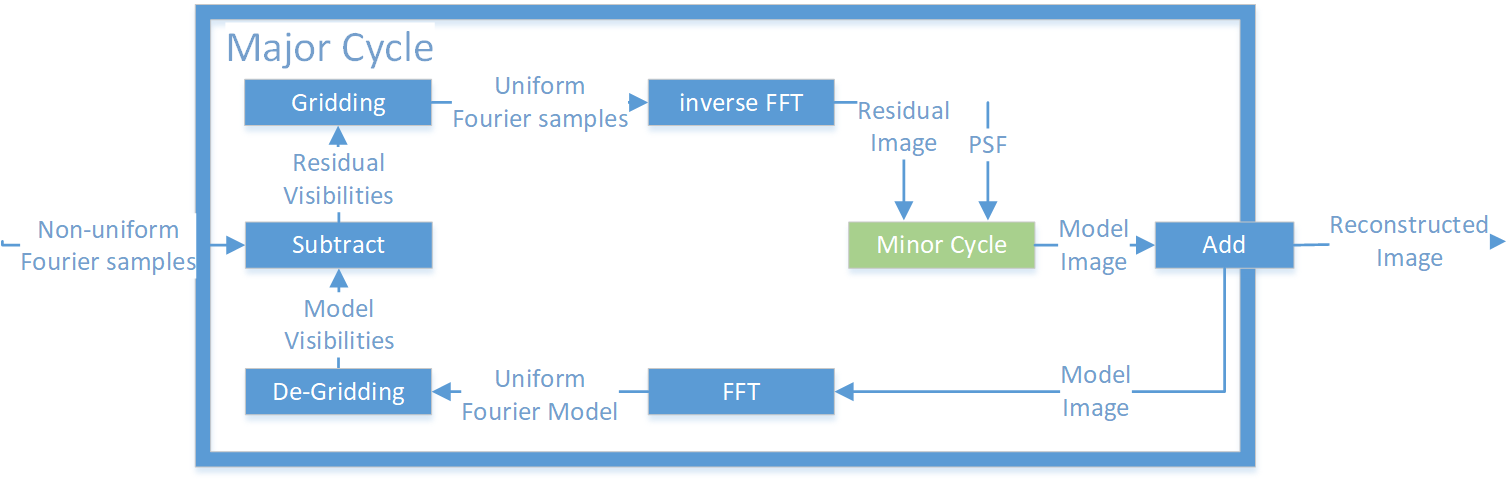
\includegraphics[width=0.8\linewidth]{./chapters/01.intro/Major-Minor4.png}
	\caption{Major/Minor cycle}
	\label{radio:major:figure}
\end{figure}

The major cycle has updated the residuals, and the deconvolution algorithm can continue. The Major cycle allows us to use an approximate $PSF$ in the deconvolution algorithm. Typically, we need several thousand Minor cycles, and between three to ten major cycles to reconstruct an image. The exact numbers depend on the observation itself.

We already discussed the Minor cycle algorithm in detail, now let us turn to the Major cycle algorithm. The Major cycle uses two steps to transform the visibilities to image space. First the gridder takes the visibilities and interpolates them on a uniform Fourier grid. Next, the inverse FFT is applied, resulting in the residual image. 

The gridding step and the Minor Cycles are the two bottlenecks in the reconstruction. The gridding step has to interpolate the visibility measurements, which generally has magnitudes more measurements than pixels. The Minor Cycle can become more expensive if the image contains a large number of complex radio source, for example several supernova-remnants. Depending on the image, it can even become more expensive than the gridding step \cite{offringa2017optimized}.

Our project focuses on the Minor cycle deconvolution algorithm. We develop two coordinate descent based deconvolution algorithm, which are used within the Major/Minor cycle architecture. The Major cycle allows us to use an approximate $PSF$ in the deconvolution. Efficient CLEAN algorithm were already developed, which use an approximation of the constant $PSF$ during deconvolution \cite{clark1980efficient}. Our hypothesis is we can approximate the constant $PSF$ further to simplify the problem for parallel and distributed deconvolution. We will develop a parallel coordinate descent deconvolution algorithm, which achieves a significant speedup with our own $PSF$ approximation scheme.

